\section*{GG Plot}

\begin{frame}
    If we create a scatter plot
    with lateral acceleration on the $x$-axis,
    and longitudinal acceleration on the $y$-axis,
    the points all fall within an ellipse.
    \begin{figure}
        \includegraphics[width=0.9\textwidth]{res/Testing GG Plot.png}
    \end{figure}
    \begin{block}{~}
        Based on this diagram,
        which driver will set the fastest laptime?
    \end{block}
\end{frame}

\begin{frame}{The Friction Ellipse}
    The friction ellipse gives the limits of the tyre's grip.
    In order to produce lateral force during a turn,
    the tyre must trade off longitudinal force.
    The characteristics of the tyre
    will affect the shape and size of the friction ellipse.
    \begin{columns}
        \column{0.45\textwidth}
        \begin{figure}
            \includegraphics[width=\textwidth]{res/Tyre Friction Ellipse.jpg}
        \end{figure}
        \column{0.55\textwidth}
        \begin{figure}
            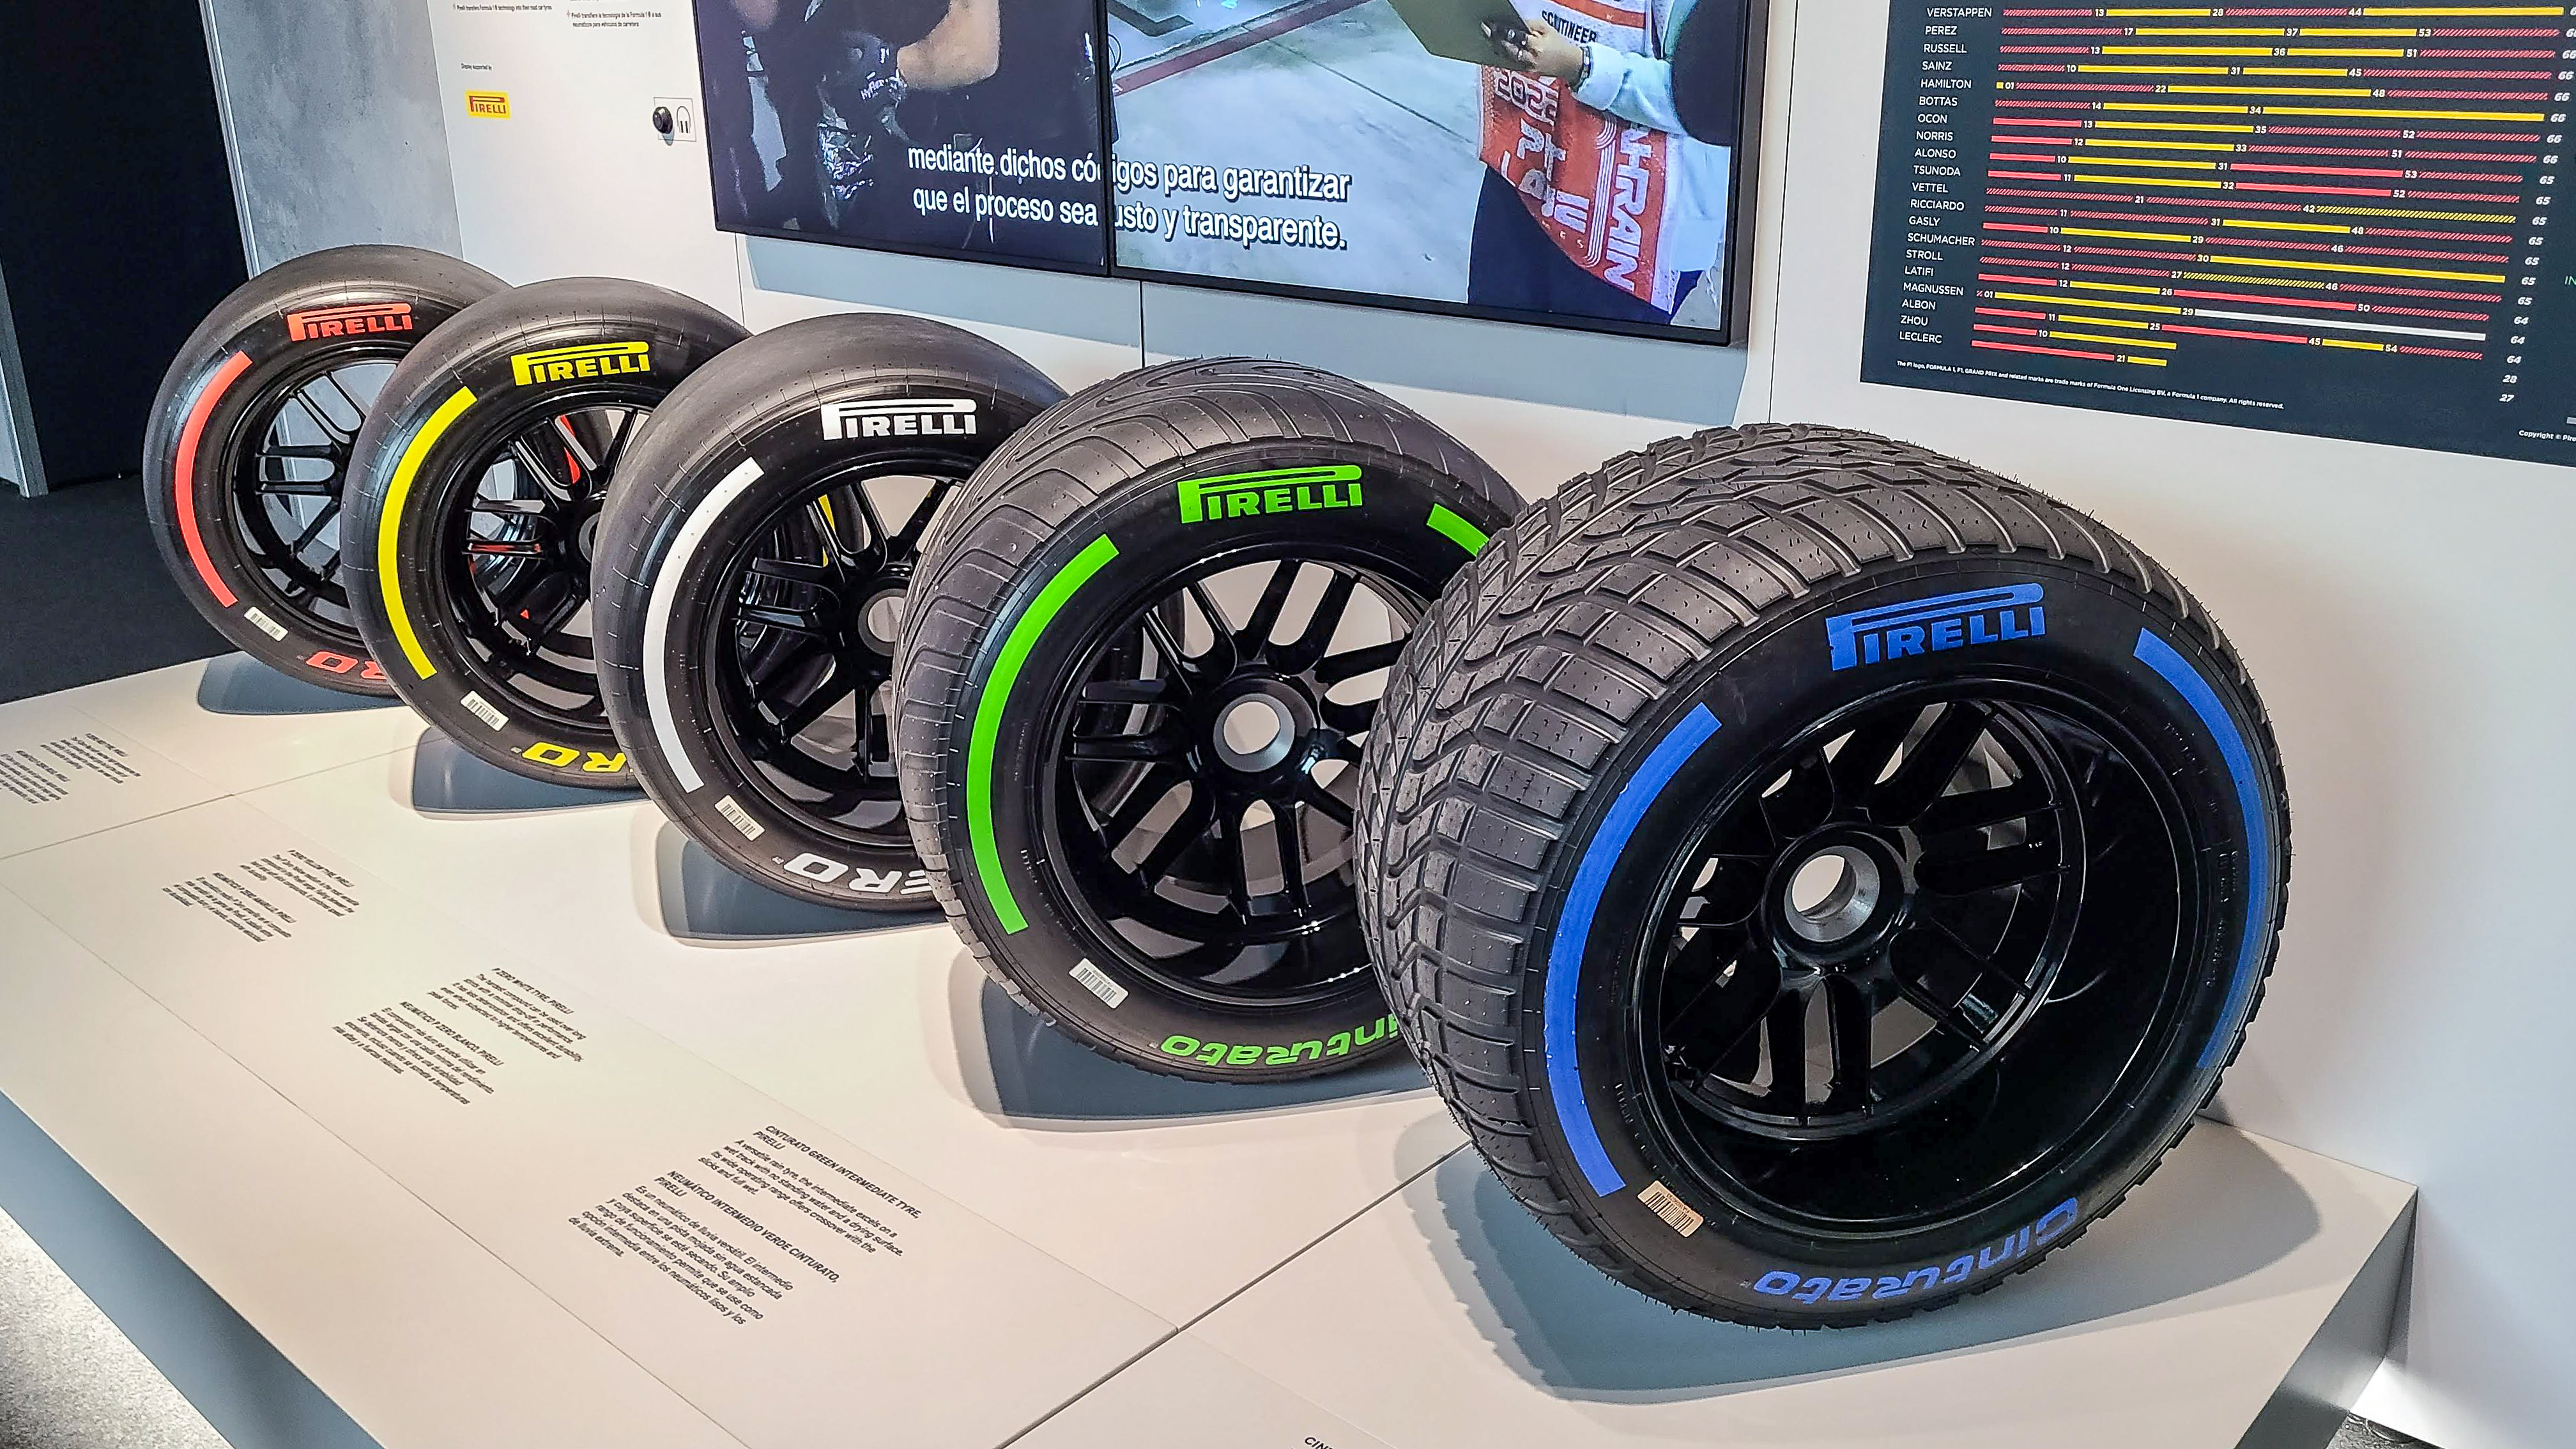
\includegraphics[width=\textwidth]{res/Formula 1 Tyres.jpg}
        \end{figure}
    \end{columns}
    \begin{block}{~}
        What will the differences be between
        the friction ellipses of the different Formula 1 tyres?
    \end{block}
\end{frame}

\begin{frame}{The GG Plot}
    \begin{columns}
        \column{0.45\textwidth}
        The friction ellipse of the tyres
        leads directly to the circular shape of the GG plot. \\
        \vspace{2ex}
        A fast driver will stay as close to the limits
        of the GG plot as possible.
        \column{0.55\textwidth}
        \begin{figure}
            \includegraphics[width=\textwidth]{res/GG Plot.png}
        \end{figure}
    \end{columns}
    \begin{block}{~}
        When looking at the GG plot of the whole car,
        it is skewed towards the braking side.
        Why is this?
    \end{block}
\end{frame}

\begin{frame}{The GGV Plot}
    The limits of the GG plot
    are influenced by the aerodynamics of the car,
    which is dependent on the car's speed.
    We can add velocity as a third axis.
    \begin{columns}
        \column{0.55\textwidth}
        \begin{figure}
            \includegraphics[width=\textwidth]{res/GGV Plot.png}
        \end{figure}
        \column{0.4\textwidth}
        \begin{block}{~}
            If we took a vertical slice of this diagram
            where lateral acceleration is zero,
            we would obtain the velocity-acceleration plot
            that we looked at last week.
        \end{block}
    \end{columns}
\end{frame}